\section{МЕТРИКИ ОЦІНКИ ЯКОСТІ}

Система рекомендацій, як інструмент, повинна виконувати поставлені
їй задачі. Як приклад візьмемо задачі із області е-коммерції, а
саме ключові показники продуктивності бізнесу (Рис. 4.1):
\begin{itemize}
    \item CR(Conversion Rate)
    \item CTR
    \item LT(Life Time)
    \item LTV(LifeTime Value)
    \item Retention
    \item User Egagement
\end{itemize}
\begin{figure}[h]
    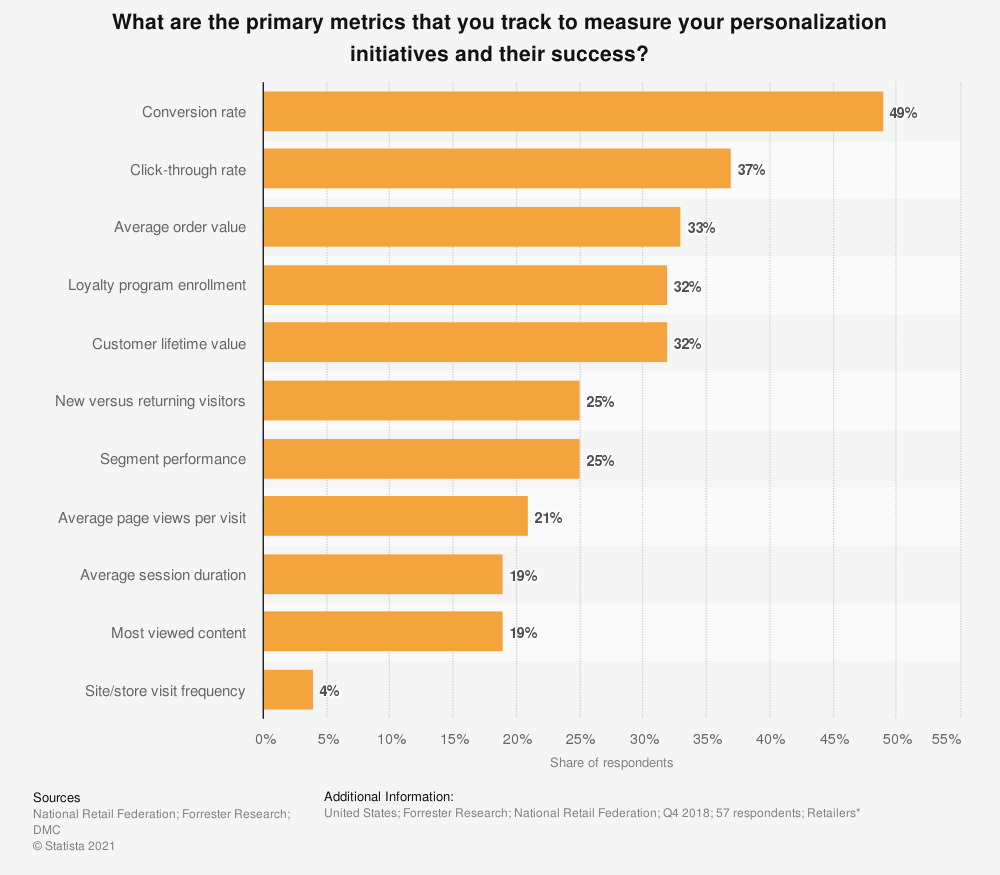
\includegraphics[width=1\textwidth]{images/E_commerce_metrics.png}
    \caption{Рейтинг популярності комерційних метрик}
    \label{fig:ecommerce_pop_metric}
\end{figure}

Найкращий спосіб визначити, чи покращує RS ці показники - провести A/B тест за допомогою відгуків користувачів.
Однак A/B тест, як правило, є дорогим і довготривалим у імплементації. Тому, перш ніж провести тест A/B, бажано
застосувати дешевший та швидший метод тестування в режимі офлайн,
щоб зменшити можливість значного падіння якості наданих рекомендацій.

Це призводить до розробки різних підходів, таких як тестування на
згенерованих даних та офлайн-оцінки, що є стандартним способом
порівняння продуктивності різних моделей. Важливо
підтримувати послідовність та рівномірність на всіх етапах,
включаючи метричний розрахунок.

\subsection{Класифікація метрик систем рекомендацій}
В силу специфіки нашої задачі, метрики системи можна умовно
поділити на групи взалежності від підходу -
\textbf{Метрики Класифікації},
\textbf{Метрики Ранжування},
\textbf{Метрики Новизни і різноманіття}. Введемо означення для опису метрик:
\begin{itemize}
    \item u  ідентифікатор користувача
    \item i  ідентифікатор об’єкта рекомендацій
    \item ${rec_k}$  список рекомендацій для користувача u із з top-k обєктів рекомендацій
    \item $rel(u)$  список релевантних обєктів для користувача u із тестового набору
    \item $rank(u,i)$  позиція i обєкту у списку рекомендацій $ rec_{k}(u)$
    \item $\mathbb{I}[\cdot] $  індикаторна функція
\end{itemize}
\subsection{Метрики класифікації}
Метрики класифікації оцінюють придатність до прийняття рішень систем рекомендацій. Вони є хорошим вибором для завдань визначення важливих або нерелевантних продуктів для користувача.

\begin{figure}
    \centering
    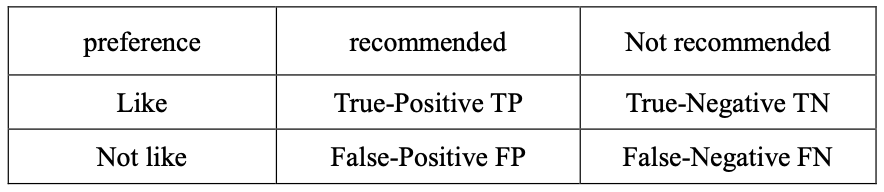
\includegraphics[width=0.7\textwidth]{images/confusion_m.png}
    \caption{Матриця помилок}
    \label{fig:conf_matrix}
\end{figure}
\subsubsection{Precision and Recall}
Метрики які широко використовуються у задачах класифікації знайшли своє використання і тут (Рис. 3.2):
\begin{align}
    Precision@k(u)=\frac{|rel(u) \cap rec_{}(u)|}{k} \\
    Precision = \frac{TP}{TP + FP}
\end{align}

\begin{align}
    Recall@k(u)=\frac{|rel(u) \cap rec_{k}(u)|}{|rel(u)|} \\
    Recall = \frac{TP}{TP+FN}
\end{align}
Precision можна інтерпретувати як частку об'єктів, що класифіковані як вірні та в той же час є вірними, і Recall показує, яка частка позитивного класу від всіх об'єктів вірного класу виявив алгоритм.
\subsubsection{F1-Score}
F1@K - це гармонічне середнє значення Precision@K і Recall@K, що допомагає спростити їх в одну метрику. Всі вищезазначені показники можна обчислити на основі матриці помилок(Рис. 3.2). Точна формула наведена нижче:
\[F1@k = 2 \times \frac{Precision@k \times Recall@k}{Precision@k + Recall@k} \]
Як ми бачимо, коефіцієнт F1 не враховує TN(True Negative). Це випадки, коли система рекомендацій не рекомендувала товар, який не має значення для користувача. Тобто метрика "сліпа" відносно певної групи обє’ктів рекомендацій. Цікавою та ідеально симетричною альтернативою є коефіцієнт кореляції Метьюса (MCC).
\subsubsection{Matthews correlation coefficient (MCC)}
Коефіцієнт кореляції Метьюса - це коефіцієнт кореляції між спостережуваною та прогнозованою бінарною класифікацією:
\[ MCC = \frac{TP\times TN - FP \times FN}{\sqrt{(TP + FP)\times(TP + FN)\times (TN+FP)\times (TN+FN)}}\]
Коли класифікатор ідеальний (FP = FN = 0) значення MCC становить 1, що вказує на ідеальну позитивну кореляцію.І навпаки, коли класифікатор завжди неправильно класифікує (TP = TN = 0), ми отримуємо значення -1, що представляє ідеальну негативну кореляцію.
\subsubsection{Hit Rate}
Приймає значення 1, коли хоч одна із рекомендацій є релевантною.
\[
    HitRate@k(u)=\mathbb{I}[|rel(u) \cap rec_{k}(u)| > 0]
\]
\subsubsection{Mean Average Precision}
Середня відносна точність(MAP) усереднюється для користувачів, і всі відмінності трапляються в розрахунку середньої точності.
\[
    AP@k(u)=\frac{1}{x}\sum\limits_{i \in rec_{k}(u)}\mathbb{I}[i \in rel(u)]Precision@rank(u,i)(u)
\]
\subsubsection{RocAuc}
Крива ROC (характеристика операційної кривої приймача) - це графік, що показує продуктивність моделі класифікації на всіх порогах класифікації (Рис. 4.3). Метрика використовує наступні складові:
\begin{itemize}
    \item TPR - True Positive Rate
          \[TPR = \frac{TP}{TP + FN}\]
    \item FPR - False Positive Rate
          \[FPR=\frac{FP}{TP + FN}\]
\end{itemize}
\begin{figure}
    \centering
    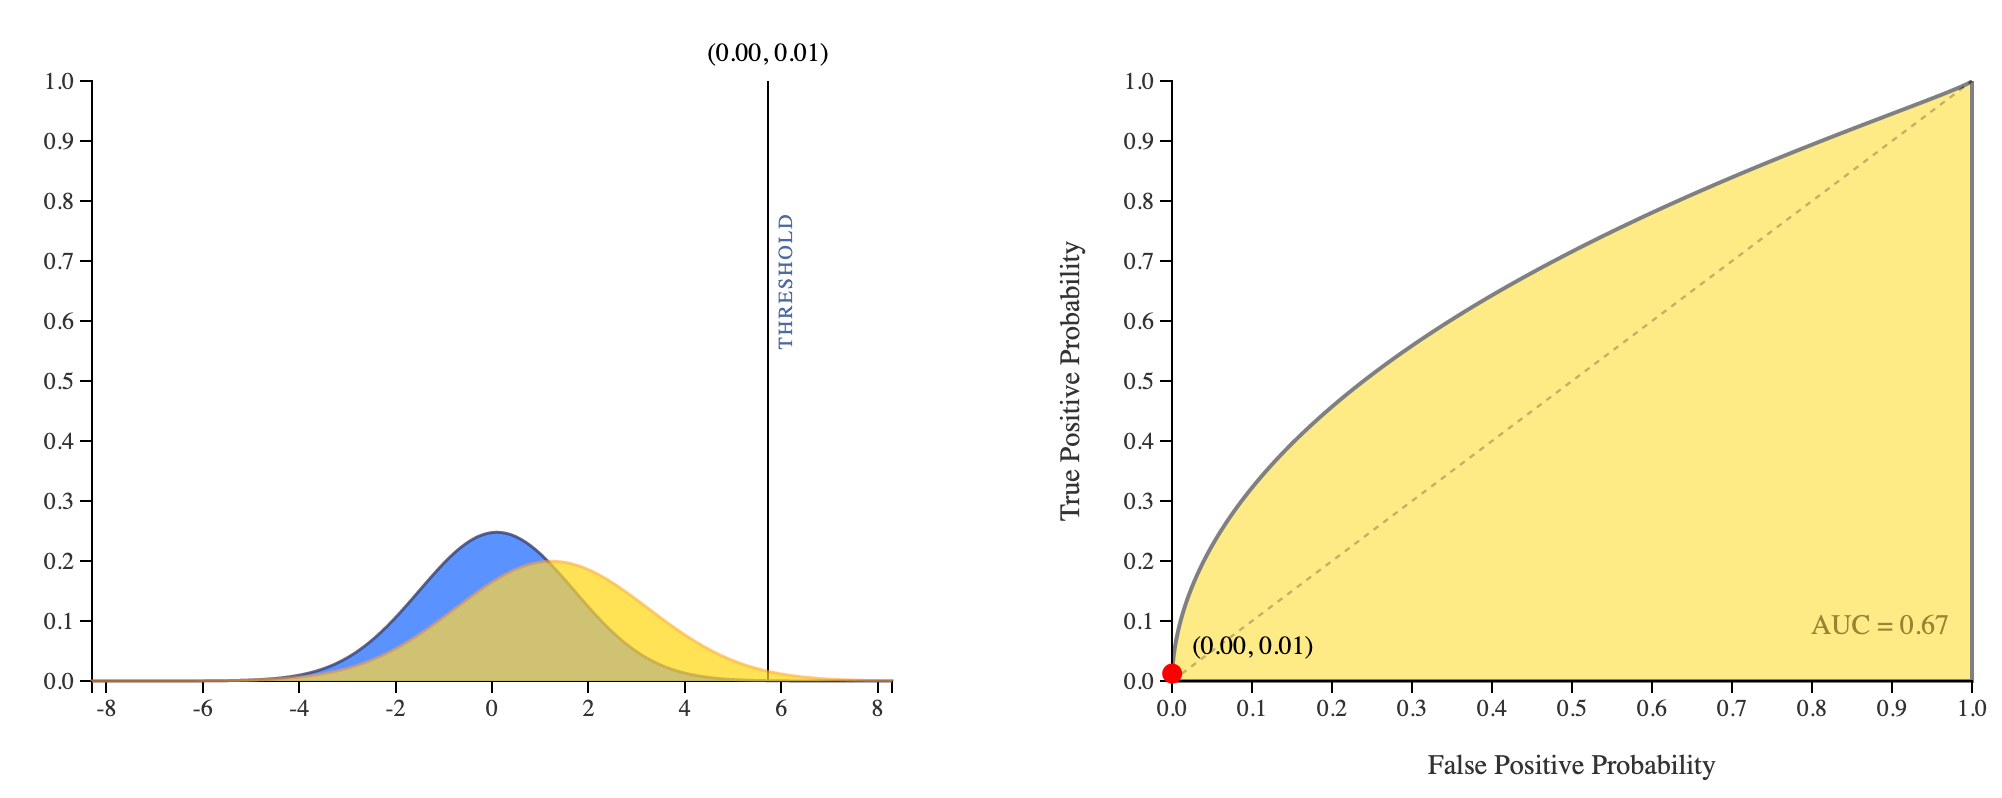
\includegraphics[width=0.8\textwidth]{images/auc_roc.png}
    \label{fig:auc_roc}
    \caption{Умовний приклад метрики ROC AUC}
\end{figure}
AUC походить від "Area under the ROC Curve". Тобто AUC вимірює всю  площу під кривою ROC від (0,0) до (1,1).AUC забезпечує сукупний показник продуктивності у всіх можливих порогах класифікації. Один із способів інтерпретації AUC - це як ймовірність того, що випадковий позитивний приклад буде оцінено більш високо, ніж випадковий негативний приклад.
AUC ціниться з наступних причин:
\begin{itemize}
    \item AUC інваріантний до масштабу. Він вимірює, наскільки добре оцінюються прогнози, а не їх абсолютні значення.
    \item AUC інваріантний до порогу чутливості. Він вимірює якість прогнозів моделі незалежно від того, який поріг класифікації обраний.
\end{itemize}

\subsection{Метрики ранжування}

\begin{figure}[h]
    \centering
    
\includegraphics[width=0.5\textwidth]{images/MLR-search-engine-example.png}
    \caption{Типова архітектура системи інформаційного пошуку}
\end{figure}

Метрики ранжування використовуются у системах рекомендації через
призму підходу як до задачі інформаційнного пошуку (Information
Retrival).

Інформаційний пошук (ІП) в обчислювальній та інформаційній науці -
це процес отримання ресурсів інформаційної системи, що
відповідають інформаційній потребі збору цих ресурсів. Пошуки
можуть базуватися на повнотекстовій або іншій індексації та на основі
вмісту. Отримання інформації - це наука пошуку інформації в
документі, пошук самих документів, а також пошук таких метаданих,
які описують дані, а також для баз даних текстів, зображень чи
звуків.

Автоматизовані системи пошуку інформації використовуються для
зменшення того, що називається перевантаженням
інформації. ІП-система - це програмна система, яка забезпечує
доступ до книг, журналів та інших документів; зберігає та керує
цими документами. Веб-пошукові системи - це найбільш помітні
ІП-програми.

\subsubsection{Cукупний інформаційний приріст}
 (Discounted Cumulative
Gain) - це показник рейтингу, який може прийняти довільні значення
релевантності.
У ІП він часто використовується для вимірювання
ефективності алгоритмів веб-пошукових систем або пов'язаних з ними
додатків. Використовуючи метрику оцінки релевантності
документів у наборі результатів пошуку, DCG вимірює корисність або
її приріст, на основі позиції елементів у списку
результатів. Чим вищий ранг обєкту у списку реезультатів тим
більше підсилюється його релевантність, а для нижчих зменшується.

Для використання метрики нам потрібно пряйняти наступні
припущення:
\begin{itemize}
    \item Існування деякої міри релевантності для елементів набору.
    \item Елементи із більш високою релевантністю приносять більше
          користі якщо вони знаходятся вище у списку (мають більш високі ранги)
\end{itemize}
% Формулювання метрики потрібно почати із $DCG$.Головна ідея - штрафувати елементи із великою релевантністю
% пропорційно до пониження їх рангу. 
Для штрафування використовуємо log reducing factor. Загальноприйнята формула для $DCG$:
\[
    DCG@k(u)=\sum_{i \in rec_{k}(u)}\frac{2ˆ{rating(u,i)} - 1}{log_{2}(rank(u,i) + 1)}
\]
$DCG$ обчислюється для одного набору документів (обєктів), для
можливості порівняння таких наборів вводять і використовують
$nDCG$, де $n$ відповідає за нормалізацію:
% \textit{ratings(u,i)} для зважування результатів. У RECSYS 
\[
    NDCG@k(u)=\frac{DCG@k(u)}{IDCG@k(u)}
\]
де $IDCG@k(u)$  (тобто $Ideal DCG$) максимально можливе значення
$DCG@k(u)$. Його ми можемо отримати у випадку ідеального
сортування набору обєктів рекомендацій довжини $k$. Для
цієї мети зазвичай використовуються рейтинги елементів із
тестового набору.
% Ми назвемо цю версію зваженою NDCG ($wNDCG$).

Також для бінарних обєктів розглядають наступну варіацію:
\[
    DCG@k(u)=\sum_{i \in rec_{k}(u)}\frac{\mathbb{I}[i \in rel(u)]}{log_{2}(rank(u,i)+1)}
\]

Можна передбачити наступні обмеження NDCG:
\begin{itemize}
    \item NDCG не штрафує за низьку релевантність самих обєктів.
          Якщо оцінки одинакові (наприклад [1, 1, 1] і  [1, 1, 1, 0])
          значення метрики буде одинакове. Потрібно використовувати
          нормування із відємним значенням для негативних елементів.
    \item Також метрика не є еффективною для малих k (набір
          рекомендації фіксованого розміру може швидко заповнюватись
          першими n елементами).
\end{itemize}
\subsubsection{Cередній взаємний ранг}
Mean Reciprocal Rank (MRR) або середній взаємній ранг - це середнє
значення зворотньої позиції (рангу) першого релевантного обєкту у
списку рекомендацій. Якщо жодних елементів не передбачано
правильно, він визначається як 0.
\[
    MRR@k(u)=\frac{1}{k}\sum_{i=1}^{|k|}\frac{1}{\min\limits_{i \in rel(u) \cap rec_{k}(u)}rank(u,i)}
\]
\subsubsection{Очікуваний взаємний ранг (Expected Reciprocal Rank)}
Припустимо, що система повертає користувачу рейтинговий список документів (рекомендацій), де ймовірність $p(q, d_{k})$, що документ задовільняє запит користувача:
\[ERR = \sum_{k=1}^{K}\frac{1}{k}p(q, d_{k}) \prod_{i=1}^{k-1}(1-p(q, d_{i}))  \]
Вибір обє’кта із певним рангом свідчить що користувач задоволений документом, ймовірність якого $p(q, d_{k})$. Також, це свідчить що всі рекомендації із вищим рейтингом  $1, ... ,k-1$ ймовірність яких $\prod_{i=1}^{k-1}(1 - p(q, d_{k}))$ не були обрані.

Для моделювання ймовірності що конкретна рекомендація буде обрана використовують так звану "редакційнку оцінку" (editorial grade) - цінність певного обєкту. В залежності від прикладної задачі можна ввести правила основані на схожості (із іншими типовими об’єктами), або передбачуванням моделі. В літературі розглядають 5 оцінок (0, 1, 2, 3, 4), де 0 це не релевантний об’єкт, а 4 дуже релевантний.
Тоді ймовірність за "редакційною оцінкою":
\[R(g):=\frac{2^{g}-1}{2^{g_{max}}}, g \in \{0, ..., g_{max}\}\]

\begin{figure}
    \centering
    \includegraphics*[width=0.3\textwidth]{images/edit_grade_prob_sample.png}
    \caption{Приклад розрахунку ймовірності для ERR}
\end{figure}

Тобто, переглядаючи результат пошуку на запит із оцінкою 3, є шанс 7/16, що користувач буде задоволений цим документом і, отже, припинить пошук, або із шансом 9/16 пошук продовжится (Рис. 4.5).

\begin{itemize}
    \item Однією приємною особливістю ERR є те, що вона завжди лежить між 0 до 1, причому 1 - найкраще. Це означає, що втрата внаслідок зіпсування будь-якого окремого прикладу обмежена.
    \item Метрика дає можливість зменшити вплив низького рангу на об’єкт. Важливість списку рекомендацій сильно падає при збільшенні його розміру (елемент із рангом 20 має множник 1/20 до своєї релевантності). ERR частково це нівелює.
\end{itemize}

\subsection{Метрики новизни і різноманітності}

Новизна та різноманітність є одним із важливих аспектів оцінки систем рекомендацій, і дозволяє більш широко підходити до оцінки кандидатів. Додатково, вказані властивості є надзвичайно корисними як із точки зору бізнесу, так і для самих користувачів. 

Прийняття кліків, переглядів або інших дій як докази прихильності користувача до контенту потребує великої долі впевненості, в тому що змодельовані оцінки справді віповідають потребам клієнта. Здебільшого, ми можем тільки надіятись що наші гіпотези будуть доказані.
Навчаючи моделі ми оперуємо лише тою частиної інформації, яку змогли зібрати.
Здебільшого, потреби користувачів є комплексні, динамічні, залежать від контексту (св’ято, пора року, час доби) і подеколи надзвичайно суперечливі.
Наприклад, перегляд мультфільму Ранго можна трактувати як прихильність до мультфільмів, або прихильність до комедій. Тому, передбачення вподобань є складним завданням, у якому не можливо досягнути ідеальної точності.

Одним із варіантів часткового вирішення таких проблем, є підхід у рекомендації надзвичайно різних по своїй природі об’єктів. Різноманіття кандидатів підвищує шанс того, що хоч одна із рекомендацій буде релевантною.
Враховуючи невизначеність щодо того, від яких характеристик залежить вподобання користувача, рекомендація фільму кожного жанру, як правило, окупається більше, ніж рекомендація, скажімо, трьох мультфільмів.

Різноманітність та новизна також знаходять мотивацію в бізнесі. Задоволеність клієнтів приносить користь бізнесу у вигляді посилення активності, доходів та лояльності клієнтів.
Крім цього, диверсифікація продукту - це відома стратегія зменшення ризику та розширення бізнесу. Більше того, це long tail sell - стратегія отримання прибутку від ринкових ніш, продаючи і отримуючи більш високу норму прибутку на дешевші продукти які важко знайти (Рис. 4.6).

Усі вищезазначені загальні міркування, звичайно, можуть бути замінені конкретними характеристиками конкретної області, ситуації та мети рекомендацій.
Наприклад, отримання списку подібних продуктів (наприклад, фотокамер) до одного, який ми зараз вибираємо, може допомогти нам уточнити наш вибір серед великого набору дуже подібних варіантів. Рекомендації можуть слугувати навігаційною допомогою в такого типу ситуації.
В інших областях є сенс споживати ті самі або дуже схожі предмети знову і знову, наприклад, покупки продуктів, одяг, тощо.

\begin{figure}
    \centering
    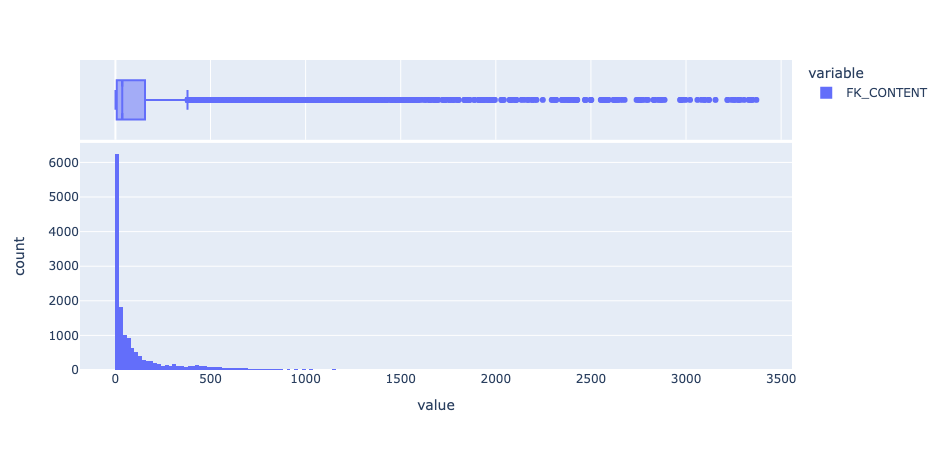
\includegraphics[width=0.8\textwidth]{images/long_tail.png}
    \caption{Типова гістрограма взаємодій користувачів, так званий "long tail" }
\end{figure}

Новизна та різноманітність суттєво різні, але пов'язані поняття (Рис. 4.7). Новизна, як правило, посилається на різницю між сучасним та минулим досвідом, тоді як різноманітність стосується внутрішніх відмінностей у елементах рекомендацій. Різноманітність, як правило, стосується набору предметів, і має відношення до того, наскільки різні предмети стосовно один одного. В основному, різноманітність оцінюється в наборі елементів, рекомендованих кожному користувачеві окремо, і, як правило, усереднюється у всіх користувачах загалом.

Загалом, варто розглянути такі наступні метрики систем рекомендацій.
\begin{figure}
    \centering
    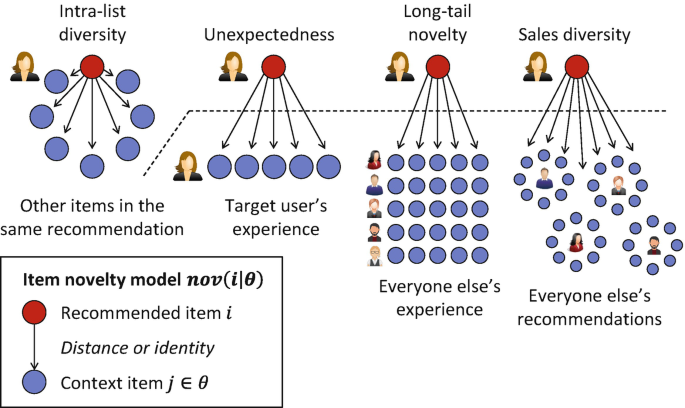
\includegraphics[width=0.7\textwidth]{images/novelity_diversity.png}
    \caption{Новизна і різноманітність у системах рекомендацій}
\end{figure}
\subsubsection{Зворотня середня частота (Mean Inverse Item Frequency)}
Використовуючи підхід ІП, частоту появи певного об’єкта у наборі взаємодій, можна інтерпретувати як міру популярності цього об’єкту. Ця частота подається у вигляді, знайомому нам із поняття інформаційної ентропії:
\[MIUF@k = -\frac{1}{|k|}\sum_{i \in k}log_{2}\frac{|U_i|}{|U|}\]
де $U_i$ множина користувачів які знайомів із об’єктом $i$. 
У перспективі така новизна на даних із довгим хвостом показує наскільки релевантний об’єкт відносно його популярності.

\subsubsection{Несподіваність (Unexpectedness)}

Несподіваність розглядають у контексті неочікуваного, але приємного досвіду.
Навідмінно від популярності, метрика цілком залежить від вподобань користувача і описує непохожість об’єктів рекомендацій із історичним досвідом користувача.

Існуює декілька варіацій Unexpectedness. Простіший варіант оцінює складність об’єктів у наборі. Під складністю розуміють наскільки не похожі об’єкти рекомендацій відносно елементів які користувач із великою ймовірністю вважає релевантними. Для створення порівняльної вибірки використовують тривіальні методи рекомендацій - вибір любимого актора, популярного реежисера, тощо.  
\[Unexpectedness@k = \frac{|K \backslash  PM|}{|K|}\]
У випадку коли у вибірці для порівняння присутні лише не відомі користувачу об’єкти: 
\[Serendipity@k = \frac{|(K \backslash  PM) \cap Rel|}{|K|}\]
де REL - це набір елементів які вважаються релевантними.
\subsubsection{Новизна (Temporal Novelity)}
Сприйняття користувача новизни також може розглядатися в межах взаємодії користувача з системою протягом деякого періоду. У цьому випадку ми визначаємо новизну як здатність систем рекомендацій не повторюватися, надаючи однакові або подібні рекомендації із часом. Ця перспектива оцінює здатність системи рекомендації генерувати нові знання про користувача та показує степінь адаптації рекомендацій до них.

\[ TN(R_u^{t}) = \frac {|R_u^{t} \bigcup_{\tau < t} R^{\tau}_u|} {|R^{t}_u|}\]
Де $R_u^{t}$ список рекомендацій у момент t.
\subsubsection{Різноманіття (Intra-List Diversity)}
Метрика оцінює наскільки відрізняються групи рекомендацій у користувачів. 
Ця оцінка є однією з найбільш вивчених у літературі, і стосується вирішення потреби користувачів у різноманітних рекомендаціях, уникаючи зайвих або монотематичних пропозицій. Метрика задається як середня парна дистанція між векторами об’єктів рекомендацій:
\[ ILD(R) = \frac{1}{|R|(|R| - 1)} \sum_{i,j \in R_u }ssim(i,j)\]  

Де у якості ssim може виступати одна із багатьох відомих метрик відстані між векторами.
\subsection*{Висновок}
На основі розглянутої літератури було відібрано і проаналізовано метрики систем рекомендацій. В результаті дослідження, метрики були поділені на 3 категорії в залежності від класу - метрики класифікації, метрики ранжування, метрики новизни і різноманіття. Для кожного класу наведено оцінки і їх опис.
